% Formato para un capítulo cualquiera

%Título del capítulo
\chapter{Arquitectura de SNSAngelGuard} 
%Sección primera
\section{Introducción}
SNSAngelGuard es una aplicación concebida como medio para realizar un ejemplo práctico sobre las investigaciones que pueden desarrollarse en una Red Social. En el presente documento, la red elegida es Facebook. Como se ha mencionado anteriormente, la base de datos de éstas investigaciones fue diseñada para albergar varias aplicaciones en las que estuvieran involucradas tambien redes sociales tales como Tuenti, Twitter, Open Social, ..., etc, por lo que la arquitectura de la base de datos no es exclusiva de SNSAngelGuard, pero sí que es totalmente compatible con Facebook.

\section{Diseño estructural}
La arquitectura se muestra en la figura 2.1. 
\bigskip
\par
\begin{figure}
\begin{center}
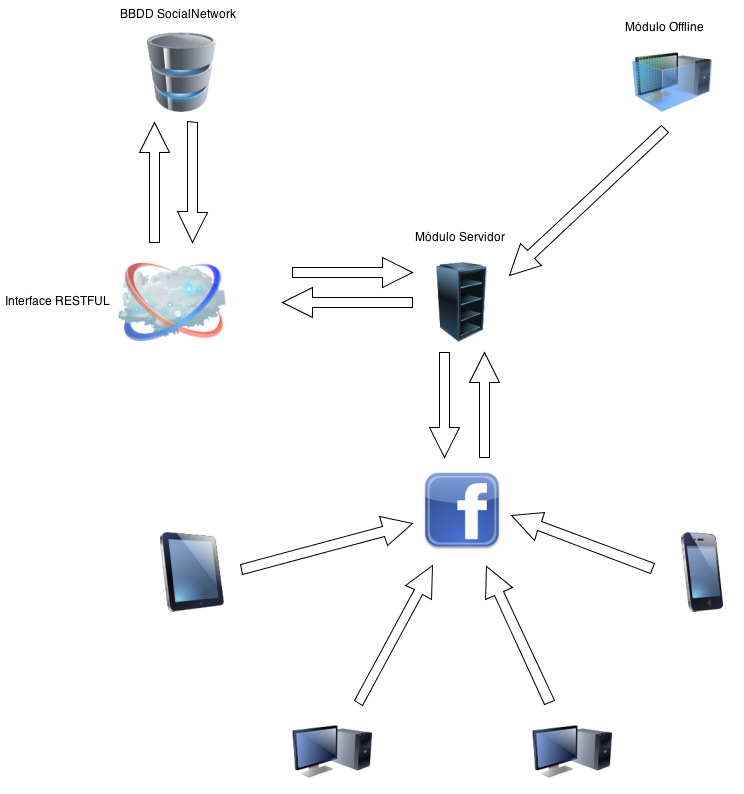
\includegraphics[width=12cm,height=10cm]{Figuras/ArchitectureSNS.png}
\end{center}
\caption{\label{Arquitectura} Arquitectura de la aplicación SNSAngelGuard}
\end{figure}
\bigskip
\par
Está conformada por una serie de módulos que se enumeran a continuación:
\begin{enumerate}
\item Base de Datos SocialNetwork: Contendrá todas las estructuras necesarias para acceder a cualquier funcionalidad de una Red Social. Guardará datos relacionados con su actividad, tales como datos a nivel personal, como pueden ser su fecha de nacimiento, su dirección, ..., etc., como datos a nivel de la propia Red Social, tales como sus amistades, sus relaciones personales con más miembros de dicha Red Social, sus comentarios en el muro, sus réplicas, enlaces a sus fotos o videos, ..., etc.
\item Interface RESTFUL: Este ente contendrá todas las estructuras necesarias para acceder a la base de datos por medio de Servicios Web. A través de éstas estructuras se creará una API que posteriormente se publicará para que todo aquel desarrollador que quiera utilizar esta base de datos pueda hacerlo como si se tratara de una API de una Red Social.
\item Módulo Servidor: Este módulo definirá una serie de estructuras que procesarán la información obtenida de los usuarios de la Red Social y, posteriormente, realizará las acciones propias de la aplicación, tales como el procesado de la información y la elaboración de informes para, posteriormente, ser enviados a los tutores del usuario en la aplicación.
\item Módulo Cliente: Está conformado por todos los dispositivos que pueden acceder a la Red Social y, a partir de ésta, ejecutar la aplicación SNSAngelGuard. Recordemos que ésta aplicación se ejecuta a través de Facebook, por lo que para acceder a ella, el usuario tendrá que tener un usuario válido dentro de ésta Red Social. Este módulo además, estará preparado para que cualquier dispositivo, sea cual fuere su naturaleza, pueda acceder a la aplicación y generar actividad a través de ella.
\item Módulo Offline: Este módulo, como su propio nombre indica, se ejecutará o podría ejecutarse, cuando un usuario no esté logueado dentro de Facebook. Estará conformado por una serie de procesos que realizan backups programados de la información del usuario en Facebook y elaborarán informes con la periodicidad indicada para cada tutor.
\end{enumerate}



\subsection{Estructura de la base de datos}
El modelo Entidad Relación que seguirá la base de datos es el que muestra la figura 2.2:
\bigskip
\par
\begin{figure}
\begin{center}
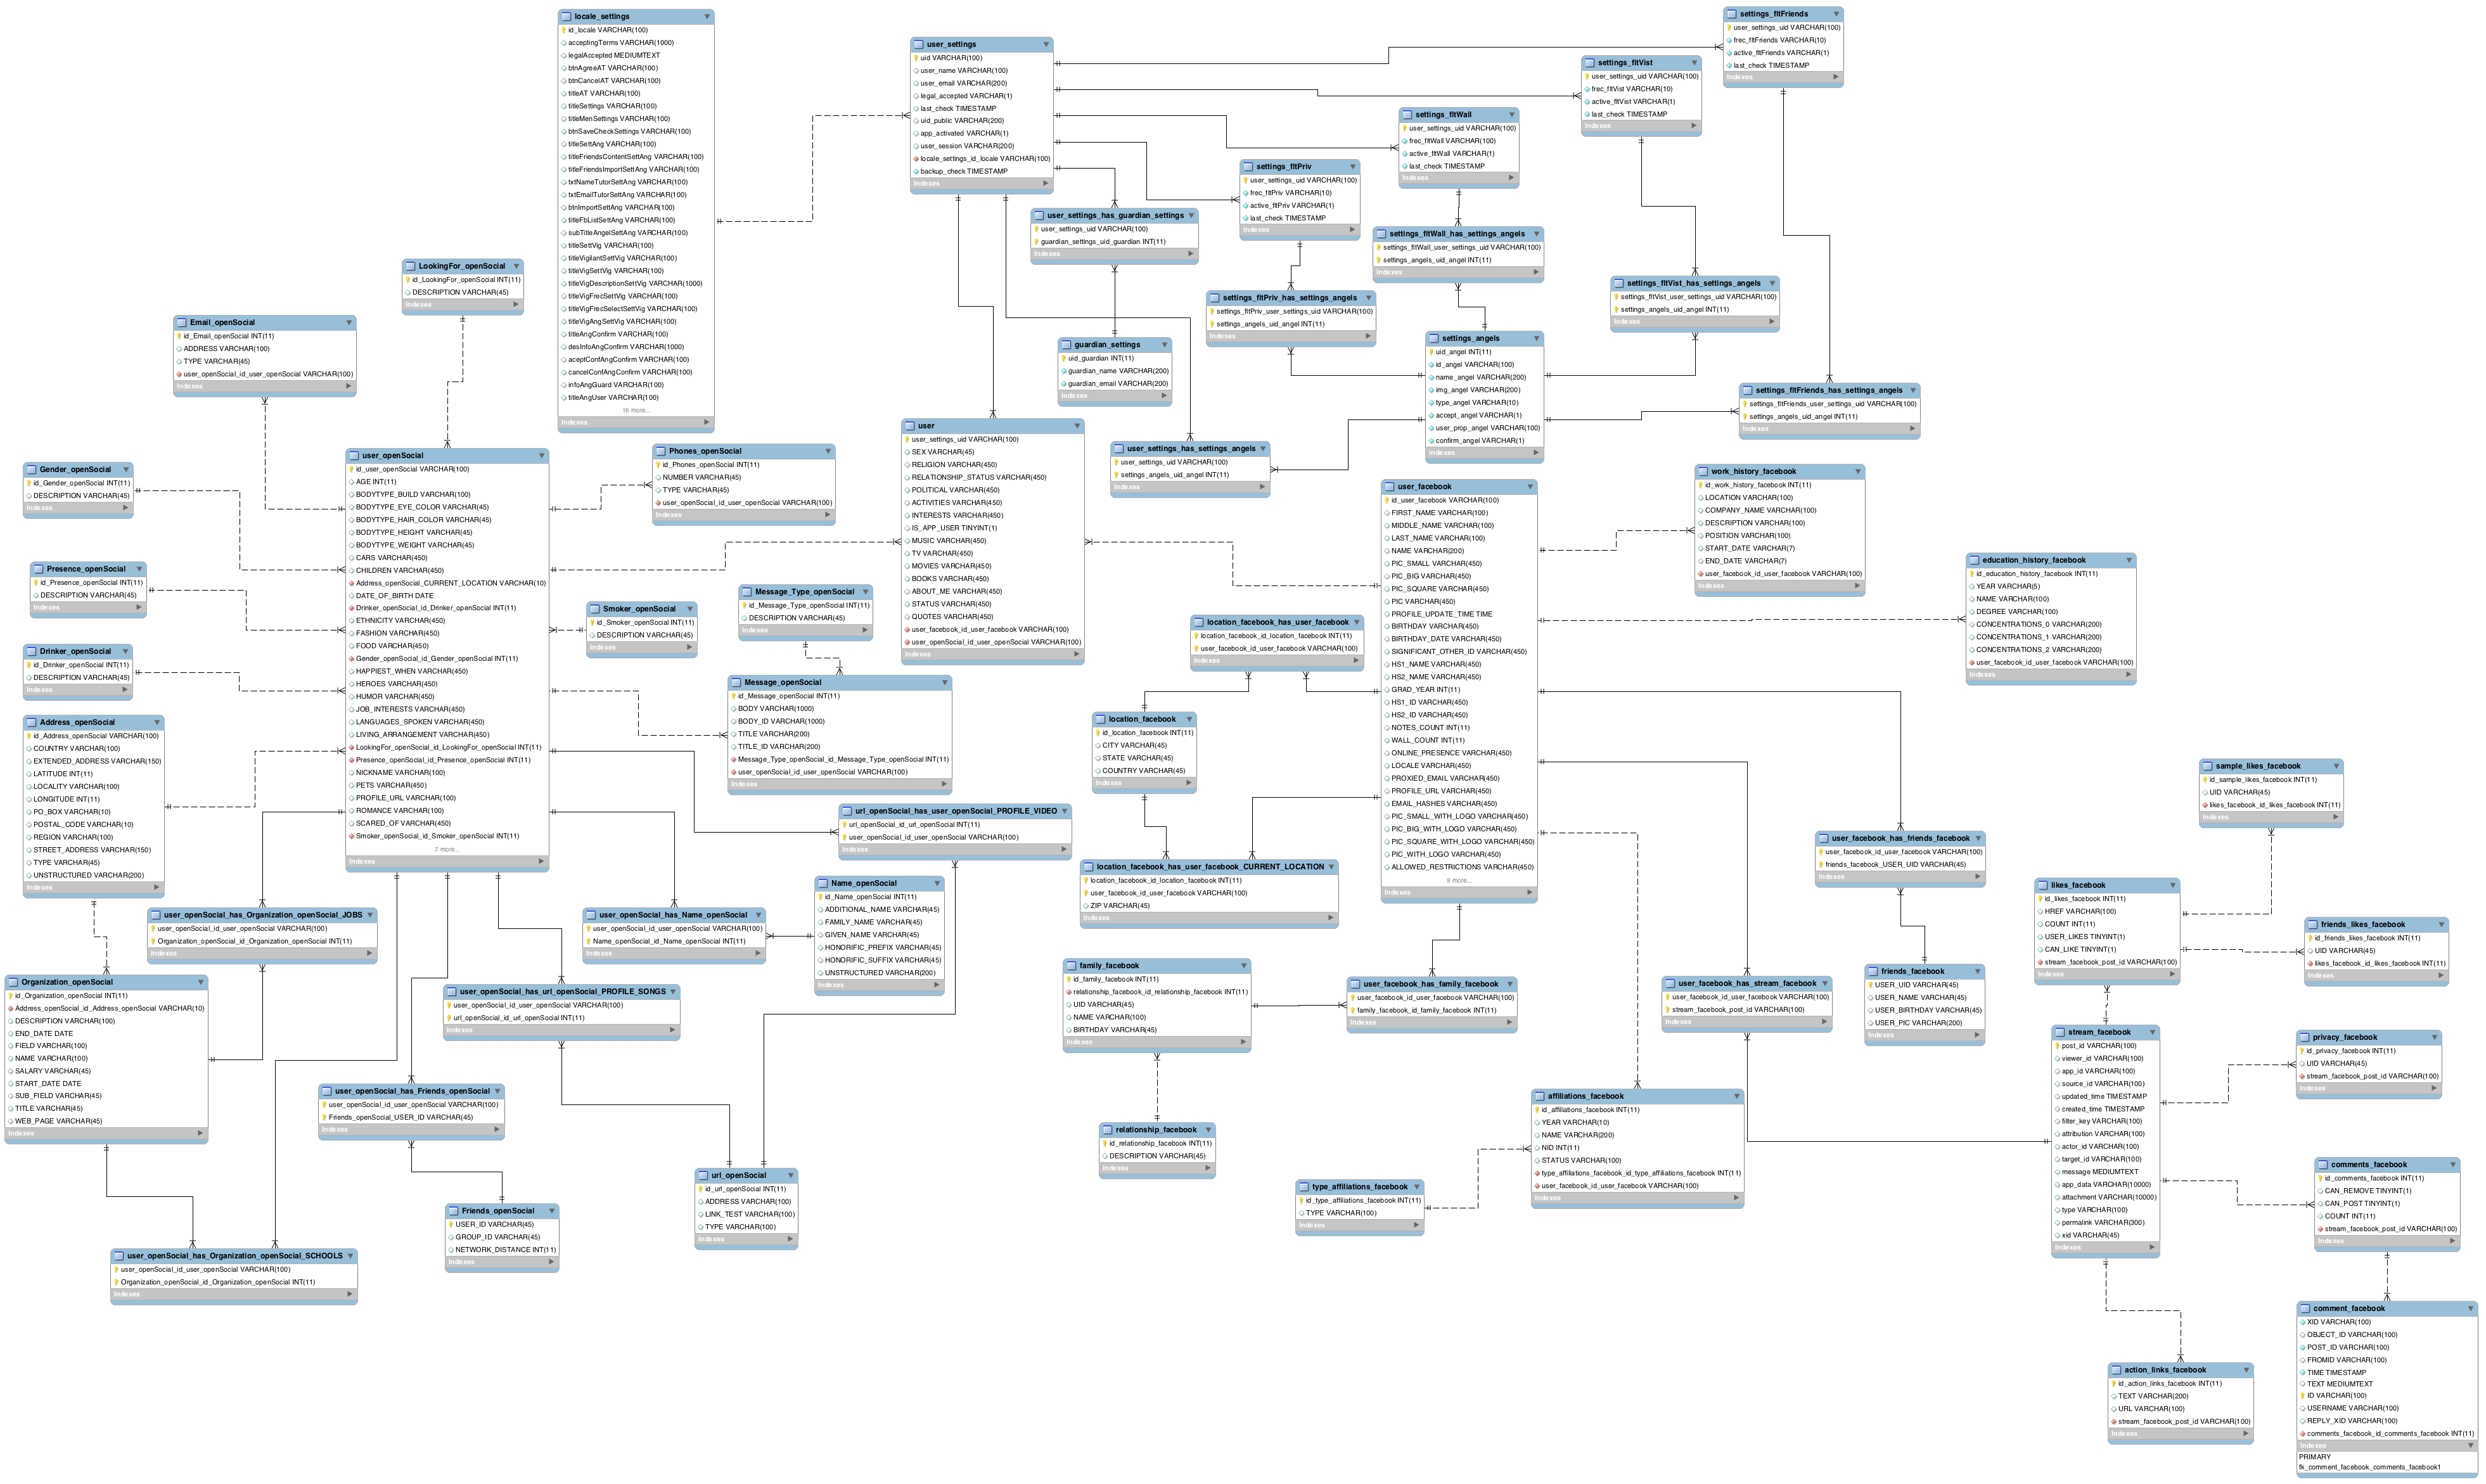
\includegraphics[width=17cm,height=19cm]{Figuras/lastModelSocialNetworkDB.png}
\end{center}
\caption{\label{ModeloER} Modelo Entidad-Relación de la base de datos de SNSAngelGuard}
\end{figure}
\bigskip
\par
La base de datos tiene tres estructuras bien definidas:
\begin{enumerate}
\item Módulo de configuración de SNSAngelGuard: En este módulo se especificarán las estructuras necesarias para la configuración de la aplicación. Contendrá estructuras para guardar los filtros\footnote[1]{Aplicaciones que analizarán la actividad social de un determinado usuario y generarán informes que serán enviados a sus ángeles.} que un usuario desee aplicar a su información, los ángeles\footnote[2]{Tutores a quienes van dirigidos los informes de la actividad social de un determinado usuario.} y la periodicidad con que éstos recibirán los informes generados por la aplicación.
\item Módulo propio de Facebook: Este módulo contendrá todas las estructuras necesarias para almacenar la información de un usuario que genera en Facebook y que será necesaria para el funcionamiento de la aplicación.
\item Módulo para otras Redes Sociales: Éste módulo contendrá las estructuras necesarias para almacenar información de otras redes sociales. Se diseñó utilizando el standar de Red Social proporcionado por OpenSocial y podrá ser adaptado a cualquier Red Social para la que se desee realizar un estudio determinado.
\end{enumerate}
\bigskip
\par
El desarrollo de ésta base de datos ha sido realizado íntegramente bajo el entorno MySQL versión 5. Para la administración, se ha utilizado el software MySQLAdmin bajo plataforma UNIX, la cual puede ser utilizada tanto en sistemas Linux, como en sistemas de la familia Macintosh.


\subsection{Módulo de comunicación con la base de datos: Interfaz RestFul}
Como se ha indicado anteriormente, el módulo de comunicación con la que el Módulo Servidor se comunicará con la base de datos, será implementado a través de Servicios Web. Para ello, se describirán las siguientes estructuras:
\begin{enumerate}
\item Módulo de Servicios Web: Será un proyecto web independiente que dará soporte a la base de datos. En él se definirán todas las estructuras necesarias para dar soporte a los servicios web que posteriormente se utilizarán en la aplicación SNSAngelGuard.
\item API propia RESTFUL: Se definirá una clase que contendrá todos los accesos a los servicios web definidos en el Módulo anterior. La razón por la que se definirá esta estructura es para que cualquier usuario, desde cualquier punto del planeta, pueda utilizar la base de datos mediante una llamada a un método remoto que le dará los datos que desee, sin tener que construir una estructura propia para el acceso a la base de datos ni tener que montar en su equipo la base de datos. Con ésta decisión se garantiza el acceso a cualquier usuario que tenga permisos para ello y la consistencia y persistencia de los datos que en ésta se almacenan, ya que ningún usuario tendrá una copia de la base de datos en su equipo, sino que trabajará remotamente con la base de datos que se defina a nivel global y cuyos parámetros de acceso serán comunicados al usuario que la quiera utilizar.
\end{enumerate}

\subsection{Módulo servidor}
El módulo servidor será la parte de la aplicación que se dedicará a procesar toda el negocio de la aplicación. Tendrá toda la responsabilidad de la aplicación y su funcionalidad. Sus objetivos serán los siguientes:
\begin{enumerate}
\item Controlar el acceso a la aplicación y gestionar la configuración de un usuario.
\item Gestionar los datos personales del usuario que se extraerán y que serán utilizados en la aplicación.
\item Analizar los datos extraídos por medio de filtros y elaborar informes.
\item Enviar los informes a los ángeles del usuario, quienes serán, en último término, los encargados de garantizar y supervisar la actividad social de un usuario en Facebook.
\end{enumerate}
\bigskip
\par
Este módulo además será el encargado de asumir las siguientes responsabilidades:
\begin{enumerate}
\item Garantizar el acceso único a la información de un usuario desde la propia aplicación.
\item Garantizar la privacidad de la información almacenada en la base de datos SocialNetwork, al igual que administrarla y gestionarla para garantizar la ejecución de los filtros definidos.
\item Analizar toda la actividad social de un usuario y comunicar cualquier anomalía definida en los filtros a sus ángeles.
\item Mantener en todo momento informado a los ángeles que se han configurado para un determinado usuario.
\item Garantizar la seguridad de la información que se envía desde la propia aplicación hasta servidores web externos a ella, tales como Gmail o Facebook.
\end{enumerate}
\bigskip
\par
Este módulo será diseñado y construido en su totalidad en el lenguaje de programación Java, combinando tanto el paradigma de Programación Orientada a Objetos, como la Programación Web en parte servidor, utilizando para ello las estructuras necesarias proporcionadas por dicho lenguaje de programación.
\subsection{Módulo cliente}
El módulo cliente será el encargado de la interfaz gráfica por el que el usuario realizará la configuración de la aplicación, seleccionando los ángeles que supervisarán su actividad social y los filtros que analizarán su información y enviarán informes de ello a dichos ángeles. Los objetivos de éste módulo serán los siguientes:
\begin{enumerate}
\item Mostrar al usuario una interfaz amigable y atractiva.
\item Integrar dicha interfaz en Facebook como una aplicación más que se ejecute desde el perfil de usuario.
\item Mostrar todos y cada uno de los amigos de Facebook para que puedan ser seleccionados por el usuario como sus ángeles.
\item Habilitar accesos desde el interfaz para poder seleccionar contactos desde cuentas de correo Gmail.
\item Habilitar las estructuras básicas para poder introducir manualmente un ángel, mediante cuadros de texto para su nombre y su dirección de correo.
\item Mostrar y controlar todos los filtros disponibles que puedan ser configurados por el usuario, mostrando además una pequeña descripción relativa a los mismos.
\end{enumerate}
\bigskip
\par
A parte de éstos objetivos, el módulo cliente se enfrentará a las siguientes responsabilidades:
\begin{enumerate}
\item Mostrar correctamente todas las estructuras necesarias para el correcto funcionamiento de la aplicación.
\item Llevar a cabo todas las validaciones de datos necesarias para que al almacenar la información de configuración, los datos estén preparados para ser procesados por el módulo servidor.
\item Controlar, en todo momento, que el usuario actual sea el único que puede acceder a su propia información de configuración.
\item Habilitar estructuras para el almacenado de la información.
\item Habilitar estructuras que informen visualmente al usuario sobre posibles errores o advertencias en el proceso de configuración. 
\item Habilitar estructuras visuales de ayuda que sirvan para aclarar posibles dudas a la hora de guardar la configuración.
\end{enumerate}
\bigskip
\par 
Todo este módulo será conformado por todas las herramientas web disponibles en la actualidad. Las principales que se han utilizado son las siguientes:
\begin{enumerate}
\item Lenguaje HTML\footnote[1]{HyperText Marckup Language, hace referencia al lenguaje de marcado predominante para la elaboración de páginas web, que se utiliza para describir y traducir la estructura y la información en forma de texto, así como complementar el texto con objetos tales como imágenes o contenido multimedia.}: Será el encargado de realizar toda la parte visual y el almacenado de la información subyacente en la arquitectura.
\item Lenguaje JavaScript\footnote[2]{Es un lenguaje de programación interpretado, que se ejecuta en la parte de cliente en una arquitectura común de Cliente-Servidor. Se utiliza implementado mediante el navegador web, permitiendo mejoras en la interfaz de usuario y en páginas web dinámicas, cuyo contenido puede variar.}: Será el encargado de realizar todas las validaciones necesarias anteriores al envío de la información y de controlar el contenido dinámico de la aplicación según las preferencias del usuario a la hora de configurar la aplicación.
\item Lenguaje JSON\footnote[3]{JavaScript Object Notation, es un formato ligero para el intercambio de datos. JSON es un subconjunto de la notación literal de objetos de JavaScript que no requiere el uso de XML.}: Realizará la tarea de intercambiar información entre el módulo cliente y el módulo servidor. También será el encargado de transferir información desde la base de datos al módulo servidor y viceversa.
\item AJAX\footnote[4]{Asynchronous JavaScript And XML, JavaScript anasíncrono y XML, es una técnica de desarrollo web para crear aplicaciones interactivas o RIA (Rich Internet Applications). Estas aplicaciones se ejecutan en el cliente, es decir, en el navegador de los usuarios mientras se mantiene la comunicación asíncrona con el servidor en segundo plano. De esta forma es posible realizar cambios sobre las páginas sin necesidad de recargarlas, lo que significa aumentar la interactividad, velocidad y usabilidad en las aplicaciones.}: Será el encargado de realizar la navegación entre paginas web pertenecientes al módulo cliente y realizar las transferencias de información entre pestañas integradas en una única página web.
\item jQuery\footnote[5]{jQuery es una biblioteca de JavaScript, creada inicialmente por John Resig, que permite simplificar la manera de interactuar con los documentos HTML, manipular el árbol DOM, manejar eventos, desarrollar animaciones y agregar interacción con la técnica AJAX a páginas web.}: Será el encargado del acceso a los elementos html de las páginas web y agrupar funcionalidad JavaScript, haciendo el código más rápido y legible.
\item JSP\footnote[6]{JavaServer Pages es una tecnología Java que permite generar contenido dinámico para web, en forma de documentos HTML, XML o de otro tipo, permitiendo la inclusión de código Java que se ejecutará directamente en servidor.}: Será el encargado de embeber las páginas html y controlar el flujo de ejecución con el servidor, realizando todas las validaciones y las transferencias de información de un módulo a otro.
\end{enumerate}

\subsection{Modulo Offline}
El Módulo Offline será el encargado de realizar los procesos de carga, validación y análisis de datos de forma automática. Se ejecutará una o varias veces al día, como tarea programada en el servidor, y realizará las siguientes acciones:
\begin{enumerate}
\item Obtener, de la base de datos SocialNetwork, la información relativa a todos los usuarios de la aplicación.
\item Por cada usuario realizará las siguientes acciones:
\begin{enumerate}
\item Descargará la nueva información que haya generado en Facebook, tal como nuevos comentarios en el muro o nuevas amistades.
\item Dependiendo de la periodicidad con que tenga configurados los filtros, realizará un análisis de la nueva información obtenida.
\item Tras realizar el análisis, informará a los ángeles los resultados obtenidos.
\item Actualizará en base de datos la fecha y la hora del momento en el que se ha realizado el proceso de actualización de la información.
\end{enumerate}
\end{enumerate}
\bigskip
\par 
Éste módulo será vital para mantener la base de datos actualizada con la última información del usuario y para realizar todas las tareas programadas por los filtros. Será desarrollado en su totalidad en Java y contendrá dos pequeños módulos:
\begin{enumerate}
\item Módulo Servidor: Éste módulo se ejecutará en el servidor web de aplicaciones mediante una conexión establecida por una tarea programada. Cuando le llega ésta llamada, pondrá en marcha todo el procedimiento descrito en el apartado anterior.
\item Tarea Programada: Dependerá del servidor o máquina física en el que se ejecute el servidor de aplicaciones. Se programará temporalmente una o varias veces diarias para poder realizar los backups de mantenimiento de la información. Será el desencadenante del proceso y sin él el Módulo Offline no se ejecutaría.
\end{enumerate} 